\documentclass[8pt, xcolor={svgnames}, hyperref={colorlinks, linkcolor=black, citecolor=amethyst, urlcolor=amethyst}]{beamer}


\usepackage[labelfont={color=amethyst,bf}]{caption}
\usetheme[progressbar=frametitle]{metropolis}
\usepackage{appendixnumberbeamer}
\usepackage{url}
\usepackage{booktabs}
\usepackage{braket}
\usepackage[scale=2]{ccicons}
\usepackage{amsfonts} 
\usepackage{amssymb}
\usepackage[english]{babel}
\colorlet{col1}{teal}
\colorlet{col2}{yellow}
\colorlet{col3}{green}
\usepackage{fontawesome}
\usepackage{subcaption}
\usepackage{multicol}
\usepackage{bm}
\usepackage{algorithm}
\usepackage{algpseudocode}
\usepackage{enumitem}

\usepackage[]{pseudo}


\usepackage{tikz}
\usetikzlibrary{positioning,arrows,calc,math,angles,quotes}
\usepackage{blochsphere}

\usetikzlibrary{arrows,automata}
\usetikzlibrary{positioning}
\usetikzlibrary{arrows.meta,
                bending,
                intersections,
                quotes,
                shapes.geometric}

\tikzset{
    state/.style={
           rectangle,
           rounded corners,
           draw=black, very thick,
           minimum height=1em,
           inner sep=2pt,
           text centered,
           },
}


\definecolor{myv}{rgb}{0.36, 0.22, 0.33}
\definecolor{gio}{rgb}{0.45, 0.31, 0.59}
\definecolor{light}{rgb}{0.8, 0.8, 1}
\definecolor{warmblack}{rgb}{0.0, 0.26, 0.26}
\definecolor{brown(web)}{rgb}{0.65, 0.16, 0.16}
\definecolor{cadmiumgreen}{rgb}{0.0, 0.42, 0.24}
\definecolor{darkmidnightblue}{rgb}{0.0, 0.2, 0.4}
\definecolor{brightube}{rgb}{0.82, 0.62, 0.91}

\definecolor{codegreen}{rgb}{0,0.6,0}
\definecolor{codegray}{rgb}{0.5,0.5,0.5}
\definecolor{codepurple}{rgb}{0.58,0,0.82}
\definecolor{backcolour}{rgb}{0.95,0.95,0.92}
\definecolor{amethyst}{rgb}{0.6, 0.33, 0.73}

\definecolor{light-gray}{gray}{0.95}
\newcommand{\code}[1]{\colorbox{light-gray}{\texttt{#1}}}
\usepackage{listings}
\lstdefinestyle{mystyle}{
    backgroundcolor=\color{backcolour},   
    commentstyle=\color{codegreen},
    keywordstyle=\color{codepurple},
    numberstyle=\tiny\color{codepurple},
    stringstyle=\color{magenta},
    basicstyle=\scriptsize,
    breakatwhitespace=false,         
    breaklines=true,                 
    captionpos=b,                    
    keepspaces=true,                 
    numbers=left,                    
    numbersep=5pt,                  
    showspaces=false,                
    showstringspaces=false,
    showtabs=false,                  
    tabsize=2
}

\lstset{style=mystyle}
\usepackage[most]{tcolorbox}
\usepackage{xcolor}

%\usepackage[citecolor = green, linkcolor = blue, bookmarks=true, urlcolor=blue,
%colorlinks=true, pagebackref=true]{hyperref}


%\usepackage{xspace}

\title{Density estimation via quantum adiabatic computing}
\subtitle{Based on \faBook\,\, \href{https://arxiv.org/abs/2303.11346}{arXiv:2303.11346}}
\date{20 April 2023}
\author[Matteo Robbiati, Juan Manuel Cruz-Martinez, Stefano Carrazza]{Matteo Robbiati, Juan Manuel Cruz-Martinez, Stefano Carrazza}
\titlegraphic{
\begin{tikzpicture}[overlay, remember picture]

\node[at=(current page.south east), anchor=south east] {%
\includegraphics[width=.18\textwidth]{figures/qibo.png} 

\includegraphics[width=.18\textwidth]{figures/unimi.png} 
\includegraphics[width=.18\textwidth]{figures/cern.png}  
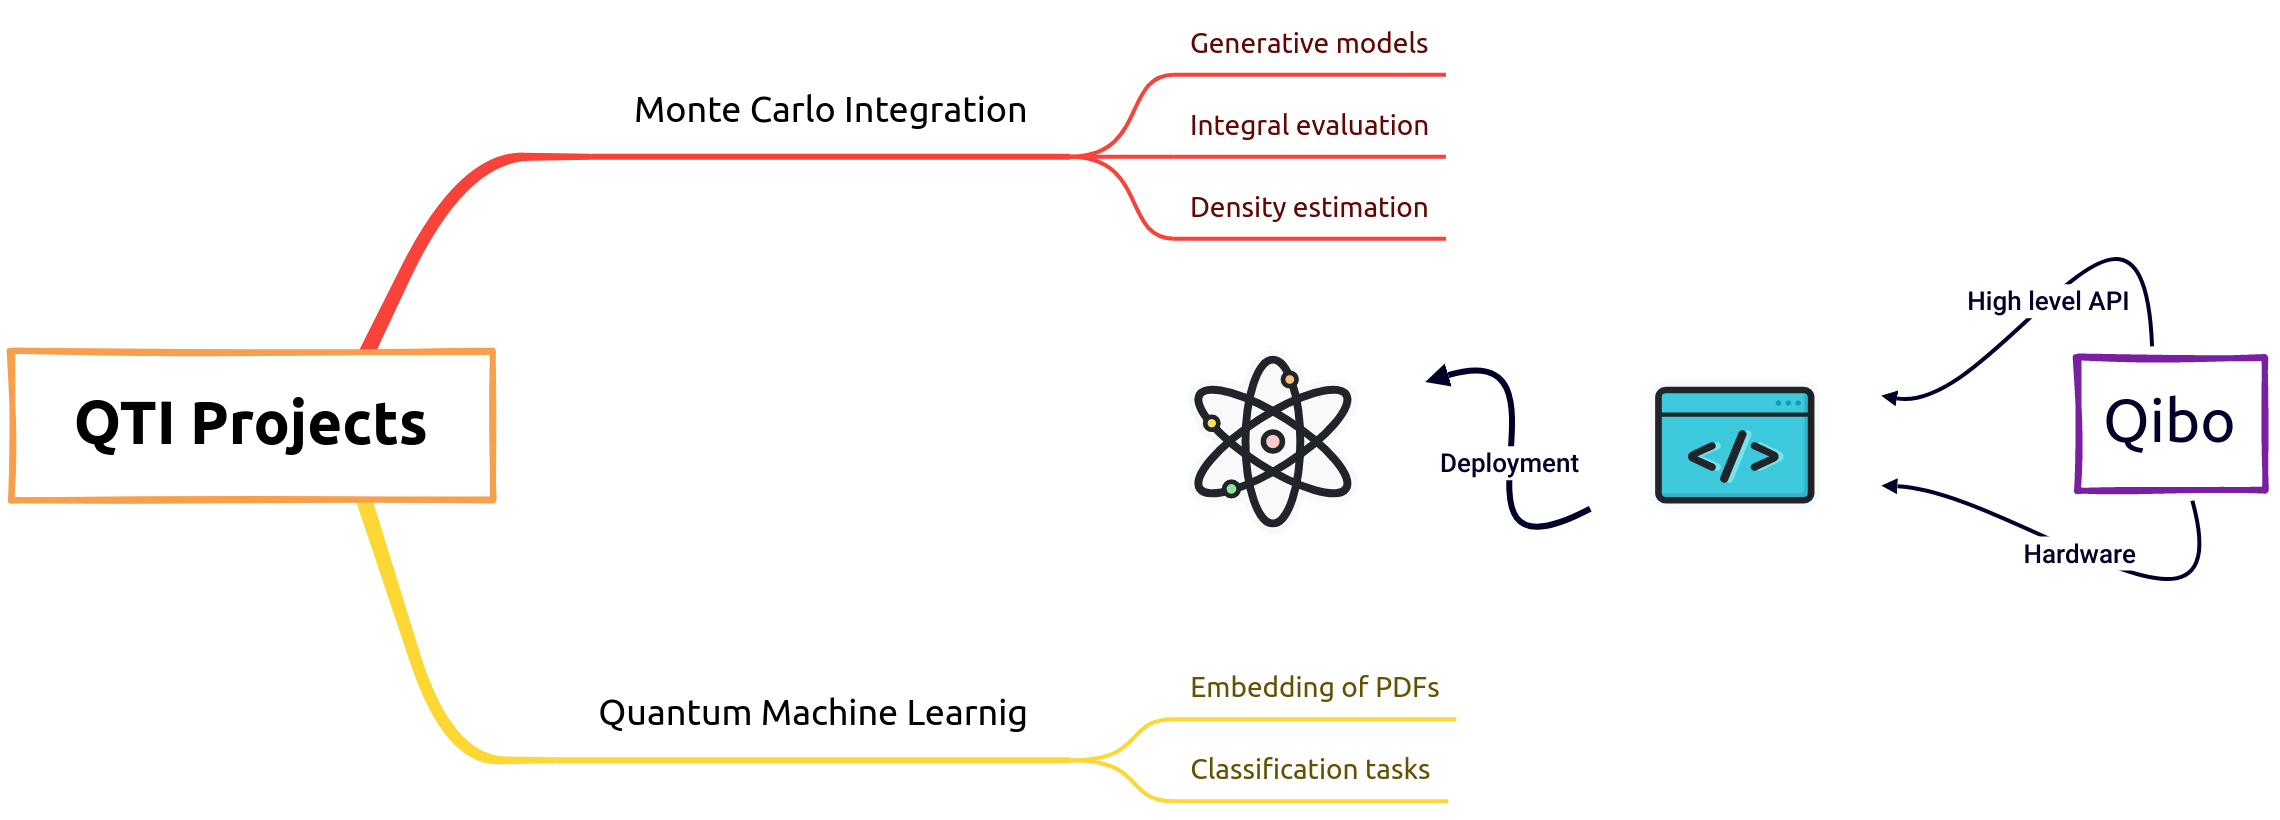
\includegraphics[width=.18\textwidth]{figures/qti.png}  
};
\end{tikzpicture}
}


\begin{document}

\maketitle

\iffalse
\section{Highlights of the previous talks}

\begin{frame}{Step back 1: Variational Quantum Circuit (VQC)}
\begin{figure}
    \includegraphics[width=0.7\textwidth]{figures/variational_model.png}
\end{figure}
\large
\begin{itemize}[noitemsep]
    \pause
    \item[\faCheckSquareO] we act on qubits states with unitaries, which we call \textbf{gates};
    \pause
    \item[\faCheckSquareO] we use \textbf{rotation} gates 
    $\exp\bigl\{-i\theta \hat{\sigma}\bigr\}$ to embed data or set parameters;
    \pause
    \item[\faCheckSquareO] we call \textbf{circuit} a sequence of gates applied 
    to a qubits system\footnote<4->{If parametrized gates are considered, we have a VQC.}; 
    \pause
    \item[\faCheckSquareO] we calculate expected values of target observables 
    through an arbitrary chosen number of circuit executions, which we call \textbf{shots}.
\end{itemize}
\end{frame}

\fi

\begin{frame}{A screenshot of Quantum Machine Learning (QML)}

\vspace{0.25cm}
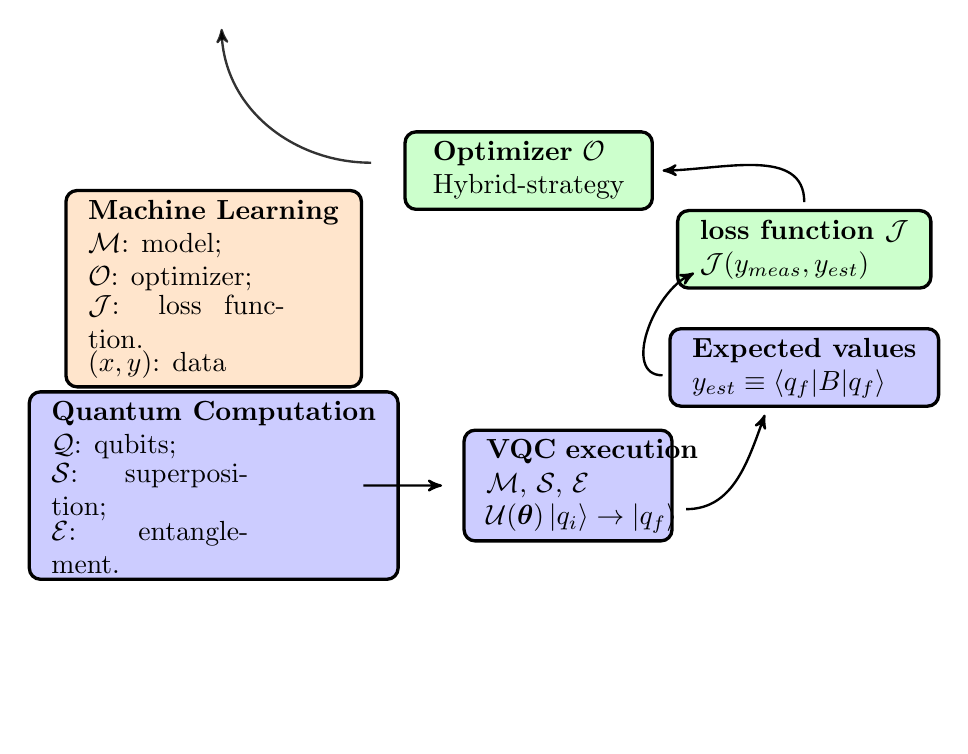
\begin{tikzpicture}[->,>=stealth']


 \node[state, fill=orange!20] (ML) 
 {\begin{tabular}{l}
 \textbf{Machine Learning}\\ 
 \parbox{2.5cm}{$\mathcal{M}$: model;}\\
 \parbox{2.5cm}{$\mathcal{O}$: optimizer;}\\
 \parbox{2.5cm}{$\mathcal{J}$: loss function.}\\
 \parbox{2.5cm}{$(x, y)$: data}
  \end{tabular}
  };
  
  \node[state,
  below of = ML,
  yshift=-1.5cm, fill=blue!20] (QC) 
 {\begin{tabular}{l}
 \textbf{Quantum Computation}\\ 
 \parbox{2.5cm}{$\mathcal{Q}$: qubits;} \\
 \parbox{2.5cm}{$\mathcal{S}$: superposition;}\\
 \parbox{2.5cm}{$\mathcal{E}$: entanglement.}
  \end{tabular}
  };
  
 \node[state,   
  text width=3cm, 
  yshift=1.5cm, 
  right of=ML, 	
  node distance=4cm, 
  anchor=center, fill=green!20] (OPT) 
 {%
 \begin{tabular}{l} 	% content
  \textbf{Optimizer $\mathcal{O}$}\\
  Hybrid-strategy
 \end{tabular}
 };
 
 \node[state,
    right of=QC,
    yshift=0cm,
    anchor=center,
    node distance=4.5cm, 	
    text width=2.5cm, fill=blue!20] (VQC) 
 {%
 \begin{tabular}{l}
  \textbf{VQC execution}\\
  $\mathcal{M}$, $\mathcal{S}$, $\mathcal{E}$ \\
  \parbox{2.8cm}{$\mathcal{U}(\bm{\theta})\ket{q_i} \to \ket{q_f}$}
 \end{tabular}
 };
 
\node[state,
  right of = VQC,
  node distance = 3cm,
  yshift=1.5cm, fill=blue!20] (NSHOT) 
 {\begin{tabular}{l}
 \textbf{Expected values}\\ 
 $y_{est} \equiv \braket{q_f|B|q_f}$
  \end{tabular}
  };
  
  \node[state,
  above of = NSHOT,
  node distance = 1.5cm,
  yshift=0cm, fill=green!20] (J) 
 {\begin{tabular}{l}
 \textbf{loss function $\mathcal{J}$}\\ 
 $\mathcal{J}(y_{meas}, y_{est})$
  \end{tabular}
  };
  

 \draw[line width=0.3mm] (1.9, -2.5)  to[out=0, in=180] (2.9, -2.5);
 \draw[line width=0.3mm] (6, -2.8)  to[out=0, in=250] (7, -1.6);
 \draw[line width=0.3mm] (5.7, -1.1)  to[out=180, in=200] (6.1, 0.2);
 \draw[line width=0.3mm] (7.5, 1.1)  to[out=90, in=0] (5.7, 1.5);
 \draw[line width=0.3mm, opacity=0.8] (2, 1.6)  to[out=180, in=270] (0.1, 3.3);
 
 \draw[line width=0.3mm, orange, opacity = 0.0] (-1.2, -1.25)  to[out=260, in=300] (4.4, -3.5);

\end{tikzpicture}
\end{frame}



\section{Introduction}

\begin{frame}{Our goal}
\large
\faArrowCircleRight\,\, QML to tackle \textbf{Monte Carlo} Integration (MCI).
\pause

\faArrowCircleRight\,\, Let's consider the integrand $g(x)$  and a dataset $\Omega$
sampled from a distribution $\rho(x)$. We are interested in calculating:
\begin{equation}
    E\bigl[g(x)\bigr] = \int_{\Omega} g(x) \rho(x) \text{d}x.
    \label{eq:MCI}
\end{equation}
\pause

\faArrowCircleRight\,\, Thus we need:
\pause
\begin{itemize}
    \item[\faDatabase] a sample of data $\Omega$ to be used for evaluating the integral;
    \pause
    \item[\faCrosshairs] a way for estimating the Probability Density Function (PDF)
    value for each given data $\rho(x)$.
    \normalsize
\end{itemize}
\vspace{0.3cm}
\pause
\begin{tcolorbox}[colback=amethyst!15, title=In this work]
    We focus on to find a \textbf{density estimation} strategy.
\end{tcolorbox}

\end{frame}

\begin{frame}{Motivation in HEP}
\large
\faArrowCircleRight\,\, Several HEP deployments exist:
\pause
  \begin{itemize}
  \item<2,3,4>[\faGear] \textbf{Monte Carlo} integration requires density estimation techniques;
  \item<3,4>[\faGear] \textbf{Parton density function} estimation (TH already worked on 
        this\footnote<3->{\href{https://arxiv.org/abs/2011.13934}{arXiv:2011.13934}});
  \item<4>[\faGear] \textbf{Anomaly detection}: if a PDF is known and punctually evaluable
        we can use this for hypotesis testing.
  \end{itemize}
  \begin{multicols}{3}
    \begin{figure}
       \uncover<2,3,4>{\includegraphics[height=3cm, width=0.33\textwidth]{figures/mci.jpeg}}%
    \end{figure}
    \begin{figure}
       \uncover<3,4>{\includegraphics[height=3cm, width=0.33\textwidth]{figures/nnpdf.jpeg}}%
    \end{figure}
    \begin{figure}
       \uncover<4>{\includegraphics[height=3cm, width=0.33\textwidth]{figures/hy_testing.jpeg}}%
    \end{figure}
\end{multicols}
\end{frame}

\begin{frame}[fragile]{Outline}
\large
\faArrowCircleRight\,\, We are going to follow these steps:
\pause
\begin{itemize}[noitemsep]
    \item[\small\faBatteryEmpty] we target the \textbf{Cumulative 
    Density Function} (CDF) of a sampled $\Omega$;
    \pause 
    \item[\small\faBatteryQuarter] we define a new \textbf{Quantum Adiabatic Machine Learning} 
    (QAML) strategy for tackling 1d fitting problems;
    \pause
    \item[\small\faBatteryHalf] we fit the CDF via QAML;
    \pause
    \item[\small\faBatteryThreeQuarters] we use parameter-shift rules for calculating 
    the PDF as derivative of the CDF; 
    \pause
    \item[\small\faBatteryFull] we validate the procedure on some test cases. 
    \pause
\end{itemize}
\vspace{0.3cm}
\begin{tcolorbox}[breakable, enhanced]
\begin{lstlisting}[language=Python, title=\textcolor{amethyst}{\faGithub\,\, Code here: \href{https://github.com/qiboteam/adiabatic-fit}{\texttt{qiboteam/adiabatic-fit}}}]
import qibo

# in some boxes like this
# we will show how to implement the QAML strategy
\end{lstlisting}
\end{tcolorbox}
\end{frame}

\section{\texttt{METHOD}: CDF fit with a VQC}

\begin{frame}{Simple case: 1d data in $\mathcal{D} = [0,1]$.}
\large
\faArrowCircleRight\,\, Each  $x\in \Omega$ can be labeled with its 
empirical CDF\footnote{\textbf{Cumulative Density Function:} after sorting the data,
$F(x)$ is calculated by counting how many elements are smaller then the target one.} value $F(x)$,
which is related to the PDF value via $\rho(x) = \frac{\text{d}F(x)}{\text{d} x}$. 

\begin{figure}
    \includegraphics[width=0.7\textwidth]{figures/pdf_cdf.pdf}
\end{figure}
\end{frame}


\begin{frame}[fragile]{Variational Quantum Circuits (VQC) as regression model}
\large
\faArrowCircleRight\,\, It is great to use a VQC as model for estimating $F$:
\pause
\begin{equation}
    \hat{F}(x; \bm{\theta}) \equiv 
    \braket{\psi_i | \mathcal{C}^{\dagger}(x;\bm{\theta})\,  \hat{\mathcal{O}} \, 
    \mathcal{C}(x;\bm{\theta}) | \psi_i},
    \label{eq:estimated_y}
\end{equation}
where $\mathcal{C}(x; \bm{\theta})$, $\mathcal{O}$ and $\psi_i$ are the respectively the 
VQC, a target observable and the initial state on which we apply $\mathcal{C}$.

\pause
\faArrowCircleRight\,\, We know how to derivate circuits, \textit{e.g.} using the
Parameter Shift Rule (PSR)\footnote<3->{\href{https://arxiv.org/abs/1811.11184}{arXiv:1811.11184}}, thanks to which we can 
calculate:
\begin{equation}
\partial_{\mu}\hat{F} = r \bigl[\hat{F}(\mu^+) - \hat{F}(\mu^-) \bigr].
\label{eq:psr}
\end{equation}  
\pause
\faArrowCircleRight\,\, In case of rotational 
gates\footnote<4->{\href{https://arxiv.org/abs/1803.00745}{arXiv:1803.00745}} 
 $\exp{\bigl\{-i\mu \hat{\sigma}\bigr\} }$ 
we have $r=0.5$, $\mu^{\pm} = \mu \pm s$ and $s=\pi/2$. 
\end{frame}

\begin{frame}[fragile]{PSR}
\large
\faArrowCircleRight\,\, We can upload $x$ into a rotation angle and calculate $\partial_x \hat{F}$.

\begin{tcolorbox}[breakable, enhanced]
\begin{lstlisting}[language=Python]
from qibo import models, gates, hamiltonians, derivative

# here you define a parametric circuit c as explained during the tutorials
# in which you upload x into the p-th rotation angle, as theta = x*PAR
# then you define an observable
h = hamiltonians.Z(nqubits=1)

# derivative with respect to x of < h >
derivative = derivative.parameter_shift(
    circuit = c,                     # parametric circuit
    hamiltonian = h,                 # target observable
    parameter_index = p,             # parameter index 
    initial_state = initial_state,   # initial state (before applying c)
    scale_factor = scale_factor)     # in this case PAR

\end{lstlisting}
\end{tcolorbox}
\pause
\vspace{0.3cm}
\begin{tcolorbox}[colback=amethyst!15, title=In a nutshell]
    We estimate the CDF using a VQC and we derivate it with the PSR for calculating the PDF.
\end{tcolorbox}
\end{frame}


\begin{frame}[fragile]{Two problems}
\large
\faArrowCircleRight\,\, We tried to fit CDFs using a VQC as QML model,
but we had two problems:
\begin{itemize}[noitemsep]
    \item[\faLineChart] by encoding $x$ into the rotation angles, 
    our results often did not retain a 
\textbf{strictly increasing monotony}.
    \item[\faChain] we need to fix $\hat{F}(0)=0$ and $\hat{F}(1)=1$, so we need
    to manipulate $\hat{F}$ in order to follow these constraints.
\end{itemize}

\faArrowCircleRight\,\, These conditions are needed if we deal with CDFs. 

\begin{figure}
    \includegraphics[width=0.7\textwidth]{figures/cdf.pdf}
\end{figure}

\end{frame}

\section{\texttt{METHOD}: Quantum Adiabatic ML}

\begin{frame}[fragile]{Adiabatic Evolution (AE) as QML model}
\large
\faArrowCircleRight\,\, Let's use an Adiabatic Evolution (AE) as model:
\begin{equation}
    H_{ad} = H_0 \bigl[1 - s(\tau; \bm{\theta})\bigr] + s(\tau; \bm{\theta}) H_1,
    \label{eq:adiabatic_evolution}
\end{equation}
\faArrowCircleRight\,\,following a scheduling $s$, depending on the evolution time $\tau\in[0,1]$
and on some variational parameters $\bm{\theta}$.
\pause
\begin{tcolorbox}[breakable, enhanced]
\begin{lstlisting}[language=Python]
# with qibo we can implement an Adiabatic Evolution via trotter formula
from qibo import models, hamiltonians, callbacks

# problem's parameters
nqubits = 1
h0 = hamiltonians.X(nqubits)
h1 = hamiltonians.Z(nqubits)
target_observable = h1

# we track the energy of h1 on the evolved ground state
energies = callbacks.Energy(target_observable)
evolution = models.AdiabaticEvolution(
    h0=h0, h1=h1, s = lambda t : t, dt=0.1, callbacks = [energies])

# calculate the evolved final state at time t=final_time
evolved_state = evolution(final_time = final_time)
\end{lstlisting}
\end{tcolorbox}

\end{frame}

\begin{frame}[fragile]{Adiabatic Evolution (AE) as QML model}
\large
\faArrowCircleRight\,\, We encode our problem into an AE by mapping 
$(x, F)$ into $(\tau, E)$: evolution time $\tau$ and target observable's energy $E$.   
\pause 

\faArrowCircleRight\,\, An AE \textbf{naturally} solves the two problems:
\pause
\begin{itemize}[noitemsep]
    \item[\faLineChart] the evolution is naturally monotonic.
    \pause
    \item[\faChain] we can fix $\hat{F}(0)=0$ and $\hat{F}(1)=1$ by chosing $H_0$ and $H_1$
    such that their ground-state energies are zero and one.
\end{itemize}

\pause
\faArrowCircleRight\,\, We want to push the Energy of $\mathcal{O}$ to approximate
the target $F$ value when $\tau$ corresponds to the target variable $x$.

\pause
\vspace{0.3cm}
\begin{tcolorbox}[colback=amethyst!15, title=Optimizing the AE]
The task becomes to optimize the scheduling parameters in order to let the 
AE pass through the training points.
\end{tcolorbox}
\end{frame}

\section{\texttt{METHOD}: Optimizing the AE}

\begin{frame}[fragile]{Optimizing the AE - ansatz and optimizer}
\large
\faArrowCircleRight\,\, We use a \textbf{CMA-ES}\footnote<1->{\href{https://arxiv.org/abs/1604.00772}{arXiv:1604.00772}} 
genetic algorithm and the following loss function:
\begin{equation}
    J_{\rm MSE} = \frac{1}{N_{\rm train}} \sum_{k = 1}^{N_{\rm train}} 
    \bigl[ F(x_k) - E_k(\bm{\theta}) \bigr]^2.
    \label{eq:loss_function}
\end{equation}
\pause
\faArrowCircleRight\,\, Thus we evolve the system using a \textbf{polynomial scheduling} 
function\footnote<2->{One is free to set a custom anstatz, \textit{e.g.} a neural 
network. With \texttt{qibo} an $s$ function is required such as $s(0)=0$ and $s(1)=1$.}:
\begin{equation}
s(t;\theta) = \frac{1}{\eta} \sum_{i=1}^{p} \theta_i x^{i}, \qquad
\text{with} \qquad \eta = \sum_{i=1}^{p} \theta_i,
\label{eq:scheduling_ansatz}
\end{equation}
\pause  
\vspace{0.1cm}
\begin{tcolorbox}[colback=amethyst!15, title=In each optimization step]
    We execute the evolution collecting $\{E_k\}    $, thanks to which we evaluate
    $J_{\rm MSE}$. Then, we update $\bm{\theta}$ according to the chosen technique.
\end{tcolorbox}
\end{frame}

\begin{frame}[fragile]{Optimizing the AE - optimizing with \texttt{qibo}}
\large
\faArrowCircleRight\,\, The optimization step is performed using \texttt{qibo}:
\begin{tcolorbox}[breakable, enhanced]
\begin{lstlisting}[language=Python]
import qibo 

# before we define a loss_evaluation function as J_MSE
def loss_evaluation(parameters): {...}

# then we use the cma optimizer provided by qibo
def optimize(force_positive=False, method="cma"):
    """Use qibo to optimize the parameters of the schedule function"""

    options = {
        "ftarget": target,              # Target loss function
        "maxiter": max_iterations,      # Maximum number of iterations
        "maxfeval": max_evals,          # Maximum number of function evaluations
    }
    
    # forcing the parameters to be positive; unused in this case.
    if force_positive:
        options["bounds"] = [0, 1e5]
        
    result = qibo.optimizers.optimize(loss_evaluation, parameters, method=method, options=options)
    return result
\end{lstlisting}
\end{tcolorbox}
\end{frame}


\begin{frame}[fragile]{A toy example with \texttt{nqubits=1} - starting point}
\large
\faArrowCircleRight\,\, \texttt{nparams=20}, \texttt{dt=0.1}, \texttt{final\_time=50}
, \texttt{target\_loss=None}
\begin{figure}
    \includegraphics[width=1\textwidth]{figures/ev0.pdf}
\end{figure}
\end{frame}

\begin{frame}[fragile]{A toy example - until $J_{\rm MSE}=10^{-1}$}
\large
\faArrowCircleRight\,\, \texttt{nparams=20}, \texttt{dt=0.1}, \texttt{final\_time=50}
, \texttt{target\_loss=1e-1}
\begin{figure}
    \includegraphics[width=1\textwidth]{figures/ev1.pdf}
\end{figure}
\end{frame}

\begin{frame}[fragile]{A toy example - until $J_{\rm MSE}=10^{-2}$}
\large
\faArrowCircleRight\,\, \texttt{nparams=20}, \texttt{dt=0.1}, \texttt{final\_time=50}
, \texttt{target\_loss=1e-2}
\begin{figure}
    \includegraphics[width=1\textwidth]{figures/ev2.pdf}
\end{figure}
\end{frame}

\begin{frame}[fragile]{A toy example - ending at $J_{\rm MSE}=10^{-4}$}
\large
\faArrowCircleRight\,\, \texttt{nparams=20}, \texttt{dt=0.1}, \texttt{final\_time=50}
, \texttt{target\_loss=1e-4}
\begin{figure}
    \includegraphics[width=1\textwidth]{figures/ev3.pdf}
\end{figure}
\end{frame}

\section{\texttt{DERIVATION}: from $\{H_j\}$ to a circuit}

\begin{frame}{Translating the AE into circuits}
\large 
 \faArrowCircleRight\,\, As previously said, we want to apply some \textbf{derivation rules}.
\pause

 \faArrowCircleRight\,\, During an \texttt{nsteps}-AE, we get \texttt{nsteps} 
 \textbf{``local time''} adiabatic hamiltonians $\{H_j\}$. 
\pause

\faArrowCircleRight\,\, Each of these can be associated with an \textbf{instantaneous} 
time evolution operator $U_j$, which at $\tau_j = j\,\text{d}t$ 
should be applied on to the state obtained in $\tau_{j-1}$.
\pause 

\faArrowCircleRight\,\, The time-evolved state $\tau_n$ is obtained as follows: 

\begin{equation}
  \ket{\psi(\tau_n)} = \prod_{j=0}^{n} U(\tau_j)\ket{\psi(\tau_{0})},
  \label{sequence} 
\end{equation}

where the initial state is the ground state of $H_0$ by construction.

\end{frame}

\begin{frame}{From a sequence to a single $U$}
\large
\faArrowCircleRight\,\, To calculate the derivative of \eqref{sequence}
is not trivial, is better to have a \textbf{single unitary} $\mathcal{C}(\tau)$ 
which sums up all the sequence needed to get the evolved state at $\tau$.
\pause

\faArrowCircleRight\,\, For doing this:
\pause
\begin{itemize}[noitemsep]
    \item[1.] we noticed that each $U_j=\exp\{-iH_j\text{d}\tau \}$ can be 
    diagonalized;
    \pause
    \item[2.] once diagonalized $\forall j$, we consider the limit
    such that $\text{d}\tau \to 0$;
    \pause
    \item[3.] thanks to which the diagonalizing element $P_j P_{j-1}^{-1}\to I$ 
    and we get:
    \begin{equation}
  \mathcal{C}(\tau) = \Lambda_{t0}
   P_t \exp \bigg\{-i t \int_{0}^{t} \hat{D}(t) \text{d}t \bigg\} P_0^{-1}, 
    \end{equation}  
    Where the $\Lambda$ factor is is used to make the determinant of $P$ be one
    and $\hat{D}$ is the diagonalized hamiltonian.
    \pause
    \item[4.] Now we have a circuit $\mathcal{C}$ after which evaluate $\hat{Z}$.
\end{itemize}

\end{frame}

\begin{frame}{From $\mathcal{C}$ to a 3-rotations circuit $\mathcal{C}_R$}
\large
\faArrowCircleRight\,\, We have a unitary 
$\mathcal{C}$, of which we can calculate the elements $c_{ij}$.
\pause 

\faArrowCircleRight\,\, The final step is to re-write this unitary in a form on 
which we can use the \textbf{parameter shift rule}. 
\pause 

\faArrowCircleRight\,\, Each unitary $\mathcal{C}\in SU(2)$ can be
written as sequence of \textbf{three rotations} using the Euler angles:
\begin{equation}
  \mathcal{C} \equiv R_z(\phi)R_x(\theta)R_z(\psi),
\end{equation}
\pause 
in which the relationships between the angles and the 
elements of $\mathcal{C}$ are:
\begin{equation}
  \begin{cases}
    \phi = \pi/2 - \text{arg}(c_{01}) - \text{arg}(c_{00}) \\
    \theta = -2\arccos(|c_{00}|) \\
    \psi = \text{arg}(c_{01}) - \pi/2 - \text{arg}(c_{00}).
  \end{cases}
\end{equation}
\pause 
\faArrowCircleRight\,\, Now we can derivate with respect to the rotation angles!

\end{frame}

\section{\texttt{DERIVATION}: derivating $\mathcal{C}_R$ via PSR}


\begin{frame}{Derivating $\mathcal{C}_R$ to get the PDF}
\large
\faArrowCircleRight\,\, I we call $\theta$ one of the three angles, we get
$\partial_{\tau} \hat{F}$ by calculating:
\begin{equation}
  \partial_{\tau} \hat{F}(\tau; \bm{\theta}) = 
  \sum_{i=1}^3 \textcolor{amethyst}{\frac{\partial \hat{F}}{\partial\theta_i}} 
  \frac{\partial \theta_i}{\partial s} \frac{\partial s}{\partial \tau},
\end{equation}
\pause
\faArrowCircleRight\,\, where the \textcolor{amethyst}{first term} 
is calculated via parameter shift rule, and the remaining 
twos can be obtained \textbf{analytically} if we use an analytical ansatz for $s$.
\pause
\vspace{0.3cm}
\begin{tcolorbox}[colback=amethyst!15, title=Summary]
\begin{itemize}[noitemsep]
    \item[\faTerminal] We fit the eCDF via QAML;
    \item[\faTerminal] we translate $\{H_j \}$ into $\mathcal{C}_R$;
    \item[\faTerminal] we derivate the result via chain rule.
\end{itemize}
\end{tcolorbox}

\end{frame}

\section{\texttt{VALIDATION:} test cases}

\begin{frame}{Test results}
\large 
\faArrowCircleRight\,\, We performed the QAML strategy to some test cases.
\pause 

\faArrowCircleRight\,\, We did it by simulating circuits both in ideal\footnote<2->{Exact
state vector simulation} and shot-noisy\footnote<2->{Sampling the frequencies from the
simulated state} way. 
\pause 

\faArrowCircleRight\,\, In the following table we collect realistic results in which we used 
$N_{\rm shots}=2\cdot 10^{5}$ shots for evaluating $\hat{F}$.
\begin{table}
  \begin{tabular}{lccccc}
  \hline \hline
    Fit function & $N_{\rm sample}$ & $p$ & $J_f$ & $N_{\rm ratio}$ & $\chi^2$\\
  \hline
    Gamma & $5 \cdot 10^4$ & $25$ & $2.9 \cdot 10^{-6}$ & $31$ & $2.2\cdot10^{-4}$ \\
    Gaussian mix & $2 \cdot 10^5$ & $30$ & $2.75 \cdot 10^{-5}$ & $31$ & $4.39 \cdot 10^{-3}$ \\
    $t$ & $5\cdot 10^4$ & $20$ & $2.1 \cdot 10^{-6}$ & $34$ & $3.4 \cdot 10^{-4}$ \\
    $s$ & $5\cdot 10^4$ & $20$ & $7.9 \cdot 10^{-6}$ & $34$ & $1.20 \cdot 10^{-3}$\\
    $y$ & $5\cdot 10^4$ & $8$ & $3.7 \cdot 10^{-6}$ & $34$ & $1.45 \cdot 10^{-3}$\\
  \hline \hline
  \end{tabular}
  \caption{\label{tab:summary}Summary. $N_{\rm shots} = 5 \cdot 10^4$.}
  \end{table}
\pause 
\faArrowCircleRight\,\, The last three elements in the table refers to a $pp\to t\bar{t}$
production.
\end{frame}

\begin{frame}[fragile]{Test 1: Gamma CDF}
\begin{figure}
  \centering
  \includegraphics[width=1\linewidth]{figures/CDF_Gamma_25_20_200000.pdf}
  \caption{We show the sample (grey hist), ideal (red line) and realistic 
  (blue line) simulation, theoretical CDF of the gamma distribution (dashed black
  line).}
\end{figure}
\end{frame}

\begin{frame}[fragile]{Test 1: Gamma PDF}
\begin{figure}
  \centering
  \includegraphics[width=1\linewidth]{figures/PDF_Gamma_25_20_200000.pdf}
  \caption{Above: data (grey hist), ideal (red) and realistic (blue) simulation,
  theoretical PDF law (dashed black line). Below: same quantities but normalized
  with respect to the true law with the addition of a second realistic simulation
  (yellow) line.}
\end{figure}
\end{frame}

\begin{frame}[fragile]{Test 2: gaussian mixture CDF}
\begin{figure}
  \centering
  \includegraphics[width=1\linewidth]{figures/CDF_Gauss_30_20_200000.pdf}
\caption{We show the sample (grey hist), ideal (red line) and realistic 
  (blue line) simulation, theoretical CDF of the gamma distribution (dashed black
  line).}
\end{figure}
\end{frame}

\begin{frame}[fragile]{Test 2: gaussian mixture PDF}
\begin{figure}
  \centering
  \includegraphics[width=1\linewidth]{figures/PDF_Gauss_30_20_200000.pdf}
    \caption{Above: data (grey hist), ideal (red) and realistic (blue) simulation,
  theoretical PDF law (dashed black line). Below: same quantities but normalized
  with respect to the true law with the addition of a second realistic simulation
  (yellow) line.}
\end{figure}
\end{frame}

\begin{frame}[fragile]{Test 3: quantum generation of $pp\to t\bar{t}$}
\faArrowCircleRight\,\, In a previous 
TH work\footnote{\href{https://arxiv.org/abs/2110.06933}{arXiv:2110.06933}} a 
sample of $10^{5}$ events for $pp\to t\bar{t}$ at a center of mass $\sqrt{s}=13$ 
TeV for LHC configuration was generated\footnote{$s$ and $t$ Mandelstam variables, $y$ rapidity.}.
\begin{figure}
  \centering
    \includegraphics[width=0.7\linewidth]{figures/qgan.png}%
\end{figure}
\end{frame}

\begin{frame}[fragile]{HEP 1: $y$ CDF}
\begin{figure}
  \centering
  \includegraphics[width=1\linewidth]{figures/CDF_y_8_20_200000.pdf}
  \caption{We show the sample (grey hist), ideal (red line) and realistic 
  (blue line) simulation, quantum GAN eCDF (yellow).}
\end{figure}
\end{frame}

\begin{frame}[fragile]{HEP 1: $y$ PDF}
\begin{figure}
  \centering
  \includegraphics[width=1\linewidth]{figures/PDF_y_8_20_200000.pdf}
  \caption{Above: data (grey hist), ideal (red) and realistic (blue) simulation. 
  Below: same quantities but normalized
  with respect to the true law with the addition of a second realistic simulation
  (yellow) line.}
\end{figure}
\end{frame}

\begin{frame}[fragile]{HEP 2: $t$ CDF}
\begin{figure}
  \centering
  \includegraphics[width=1\linewidth]{figures/CDF_t_20_20_200000.pdf}
  \caption{We show the sample (grey hist), ideal (red line) and realistic 
  (blue line) simulation, quantum GAN eCDF (yellow).}
\end{figure}
\end{frame}

\begin{frame}[fragile]{HEP 2: $t$ PDF}
\begin{figure}
  \centering
  \includegraphics[width=1\linewidth]{figures/PDF_t_20_20_200000.pdf}
  \caption{Above: data (grey hist), ideal (red) and realistic (blue) simulation. 
  Below: same quantities but normalized
  with respect to the true law with the addition of a second realistic simulation
  (yellow) line.}
\end{figure}
\end{frame}

\begin{frame}[fragile]{HEP 3: $s$ CDF}
\begin{figure}
  \centering
  \includegraphics[width=1\linewidth]{figures/CDF_s_20_20_200000.pdf}
  \caption{We show the sample (grey hist), ideal (red line) and realistic 
  (blue line) simulation, quantum GAN eCDF (yellow).}
\end{figure}
\end{frame}

\begin{frame}[fragile]{HEP 3: $s$ PDF}
\begin{figure}
  \centering
  \includegraphics[width=1\linewidth]{figures/PDF_s_20_20_200000.pdf}
  \caption{Above: data (grey hist), ideal (red) and realistic (blue) simulation. 
  Below: same quantities but normalized
  with respect to the true law with the addition of a second realistic simulation
  (yellow) line.}
\end{figure}
\end{frame}

\section{Outlook and references}

\begin{frame}{Outlook}
\large
\faArrowCircleRight\,\, Open roads:
\pause
\begin{itemize}
  \item[\faExternalLink] multi-dimensional\footnote<2->{In case of \textit{iid} 
  random variables this model can be used individually for each dimension.} PDFs
  : \textcolor{amethyst}{\textit{how to preserve correlations?
  how to exploit multi-qubits hamiltonians?}}
  \pause
  \item[\faExternalLink] hardware deployment: \textcolor{amethyst}{\textit{can a NISQ device be used for this?
  what is the speed-up advantage when running the QAML on annealers?}}
  \pause
  \item[\faExternalLink] use the QAML strategy for integrating, \textit{e.g.} 
  deploying of a new NNPDF feature;
  \pause
  \item[\faExternalLink] anomaly detection applications of the QAML algorithm.
\end{itemize}
\end{frame}

\begin{frame}{Some references}
\large
\faArrowCircleRight\,\, We leave some references and links thanks to which you can use our codes and read more about the project:

\begin{multicols}{2}
    
\begin{itemize}
\item[\faCode] open-access codes for personal coding or contributing:
    \begin{itemize}[noitemsep]
        \item[\faGithub]  \href{https://github.com/qiboteam/qibo}{the \texttt{qibo} package};
        \item[\faGithub]  \href{https://github.com/qiboteam/qibolab}{the \texttt{qibolab} package};
        \item[\faGithub]  \href{https://github.com/qiboteam/qibocal}{the \texttt{qibocal} package};
    \end{itemize}
 \vspace{1cm}

\item[\faBook] our official \href{https://qibo.science/}{webpage}, with the following documentations:
    \begin{itemize}[noitemsep]
        \item[\faLeanpub]  \href{https://qibo.science/docs/qibo/stable}{the \texttt{qibo} docs};
        \item[\faLeanpub]  \href{https://qibo.science/docs/qibolab/stable}{the \texttt{qibolab} docs};
        \item[\faLeanpub]  \href{https://qibo.science/docs/qibocal/stable}{the \texttt{qibocal} docs};
    \end{itemize}
\end{itemize}
\end{multicols}

The code is open-source and available \href{https://github.com/qiboteam/adiabatic-fit}{here!}
\end{frame}


\end{document}
